
%% bare_conf.tex
%% V1.3
%% 2007/01/11
%% by Michael Shell
%% See:
%% http://www.michaelshell.org/
%% for current contact information.
%%
%% This is a skeleton file demonstrating the use of IEEEtran.cls
%% (requires IEEEtran.cls version 1.7 or later) with an IEEE conference paper.
%%
%% Support sites:
%% http://www.michaelshell.org/tex/ieeetran/
%% http://www.ctan.org/tex-archive/macros/latex/contrib/IEEEtran/
%% and
%% http://www.ieee.org/

%%*************************************************************************
%% Legal Notice:
%% This code is offered as-is without any warranty either expressed or
%% implied; without even the implied warranty of MERCHANTABILITY or
%% FITNESS FOR A PARTICULAR PURPOSE! 
%% User assumes all risk.
%% In no event shall IEEE or any contributor to this code be liable for
%% any damages or losses, including, but not limited to, incidental,
%% consequential, or any other damages, resulting from the use or misuse
%% of any information contained here.
%%
%% All comments are the opinions of their respective authors and are not
%% necessarily endorsed by the IEEE.
%%
%% This work is distributed under the LaTeX Project Public License (LPPL)
%% ( http://www.latex-project.org/ ) version 1.3, and may be freely used,
%% distributed and modified. A copy of the LPPL, version 1.3, is included
%% in the base LaTeX documentation of all distributions of LaTeX released
%% 2003/12/01 or later.
%% Retain all contribution notices and credits.
%% ** Modified files should be clearly indicated as such, including  **
%% ** renaming them and changing author support contact information. **
%%
%% File list of work: IEEEtran.cls, IEEEtran_HOWTO.pdf, bare_adv.tex,
%%                    bare_conf.tex, bare_jrnl.tex, bare_jrnl_compsoc.tex
%%*************************************************************************

% *** Authors should verify (and, if needed, correct) their LaTeX system  ***
% *** with the testflow diagnostic prior to trusting their LaTeX platform ***
% *** with production work. IEEE's font choices can trigger bugs that do  ***
% *** not appear when using other class files.                            ***
% The testflow support page is at:
% http://www.michaelshell.org/tex/testflow/



% Note that the a4paper option is mainly intended so that authors in
% countries using A4 can easily print to A4 and see how their papers will
% look in print - the typesetting of the document will not typically be
% affected with changes in paper size (but the bottom and side margins will).
% Use the testflow package mentioned above to verify correct handling of
% both paper sizes by the user's LaTeX system.
%
% Also note that the "draftcls" or "draftclsnofoot", not "draft", option
% should be used if it is desired that the figures are to be displayed in
% draft mode.
%
\documentclass[10pt, conference]{IEEEtran}
% Add the compsocconf option for Computer Society conferences.
%
% If IEEEtran.cls has not been installed into the LaTeX system files,
% manually specify the path to it like:
% \documentclass[conference]{../sty/IEEEtran}





% Some very useful LaTeX packages include:
% (uncomment the ones you want to load)


% *** MISC UTILITY PACKAGES ***
%
%\usepackage{ifpdf}
% Heiko Oberdiek's ifpdf.sty is very useful if you need conditional
% compilation based on whether the output is pdf or dvi.
% usage:
% \ifpdf
%   % pdf code
% \else
%   % dvi code
% \fi
% The latest version of ifpdf.sty can be obtained from:
% http://www.ctan.org/tex-archive/macros/latex/contrib/oberdiek/
% Also, note that IEEEtran.cls V1.7 and later provides a builtin
% \ifCLASSINFOpdf conditional that works the same way.
% When switching from latex to pdflatex and vice-versa, the compiler may
% have to be run twice to clear warning/error messages.






% *** CITATION PACKAGES ***
%
%\usepackage{cite}
% cite.sty was written by Donald Arseneau
% V1.6 and later of IEEEtran pre-defines the format of the cite.sty package
% \cite{} output to follow that of IEEE. Loading the cite package will
% result in citation numbers being automatically sorted and properly
% "compressed/ranged". e.g., [1], [9], [2], [7], [5], [6] without using
% cite.sty will become [1], [2], [5]--[7], [9] using cite.sty. cite.sty's
% \cite will automatically add leading space, if needed. Use cite.sty's
% noadjust option (cite.sty V3.8 and later) if you want to turn this off.
% cite.sty is already installed on most LaTeX systems. Be sure and use
% version 4.0 (2003-05-27) and later if using hyperref.sty. cite.sty does
% not currently provide for hyperlinked citations.
% The latest version can be obtained at:
% http://www.ctan.org/tex-archive/macros/latex/contrib/cite/
% The documentation is contained in the cite.sty file itself.






% *** GRAPHICS RELATED PACKAGES ***
%
\ifCLASSINFOpdf
  % \usepackage[pdftex]{graphicx}
  % declare the path(s) where your graphic files are
  % \graphicspath{{../pdf/}{../jpeg/}}
  % and their extensions so you won't have to specify these with
  % every instance of \includegraphics
  % \DeclareGraphicsExtensions{.pdf,.jpeg,.png}
\else
  % or other class option (dvipsone, dvipdf, if not using dvips). graphicx
  % will default to the driver specified in the system graphics.cfg if no
  % driver is specified.
  % \usepackage[dvips]{graphicx}
  % declare the path(s) where your graphic files are
  % \graphicspath{{../eps/}}
  % and their extensions so you won't have to specify these with
  % every instance of \includegraphics
  % \DeclareGraphicsExtensions{.eps}
\fi
% graphicx was written by David Carlisle and Sebastian Rahtz. It is
% required if you want graphics, photos, etc. graphicx.sty is already
% installed on most LaTeX systems. The latest version and documentation can
% be obtained at: 
% http://www.ctan.org/tex-archive/macros/latex/required/graphics/
% Another good source of documentation is "Using Imported Graphics in
% LaTeX2e" by Keith Reckdahl which can be found as epslatex.ps or
% epslatex.pdf at: http://www.ctan.org/tex-archive/info/
%
% latex, and pdflatex in dvi mode, support graphics in encapsulated
% postscript (.eps) format. pdflatex in pdf mode supports graphics
% in .pdf, .jpeg, .png and .mps (metapost) formats. Users should ensure
% that all non-photo figures use a vector format (.eps, .pdf, .mps) and
% not a bitmapped formats (.jpeg, .png). IEEE frowns on bitmapped formats
% which can result in "jaggedy"/blurry rendering of lines and letters as
% well as large increases in file sizes.
%
% You can find documentation about the pdfTeX application at:
% http://www.tug.org/applications/pdftex





% *** MATH PACKAGES ***
%
%\usepackage[cmex10]{amsmath}
% A popular package from the American Mathematical Society that provides
% many useful and powerful commands for dealing with mathematics. If using
% it, be sure to load this package with the cmex10 option to ensure that
% only type 1 fonts will utilized at all point sizes. Without this option,
% it is possible that some math symbols, particularly those within
% footnotes, will be rendered in bitmap form which will result in a
% document that can not be IEEE Xplore compliant!
%
% Also, note that the amsmath package sets \interdisplaylinepenalty to 10000
% thus preventing page breaks from occurring within multiline equations. Use:
%\interdisplaylinepenalty=2500
% after loading amsmath to restore such page breaks as IEEEtran.cls normally
% does. amsmath.sty is already installed on most LaTeX systems. The latest
% version and documentation can be obtained at:
% http://www.ctan.org/tex-archive/macros/latex/required/amslatex/math/





% *** SPECIALIZED LIST PACKAGES ***
%
%\usepackage{algorithmic}
% algorithmic.sty was written by Peter Williams and Rogerio Brito.
% This package provides an algorithmic environment fo describing algorithms.
% You can use the algorithmic environment in-text or within a figure
% environment to provide for a floating algorithm. Do NOT use the algorithm
% floating environment provided by algorithm.sty (by the same authors) or
% algorithm2e.sty (by Christophe Fiorio) as IEEE does not use dedicated
% algorithm float types and packages that provide these will not provide
% correct IEEE style captions. The latest version and documentation of
% algorithmic.sty can be obtained at:
% http://www.ctan.org/tex-archive/macros/latex/contrib/algorithms/
% There is also a support site at:
% http://algorithms.berlios.de/index.html
% Also of interest may be the (relatively newer and more customizable)
% algorithmicx.sty package by Szasz Janos:
% http://www.ctan.org/tex-archive/macros/latex/contrib/algorithmicx/
\usepackage{amsmath}
\usepackage{centernot}
\usepackage{tikz}
\usepackage{xspace}

% *** ALIGNMENT PACKAGES ***
%
%\usepackage{array}
% Frank Mittelbach's and David Carlisle's array.sty patches and improves
% the standard LaTeX2e array and tabular environments to provide better
% appearance and additional user controls. As the default LaTeX2e table
% generation code is lacking to the point of almost being broken with
% respect to the quality of the end results, all users are strongly
% advised to use an enhanced (at the very least that provided by array.sty)
% set of table tools. array.sty is already installed on most systems. The
% latest version and documentation can be obtained at:
% http://www.ctan.org/tex-archive/macros/latex/required/tools/


%\usepackage{mdwmath}
%\usepackage{mdwtab}
% Also highly recommended is Mark Wooding's extremely powerful MDW tools,
% especially mdwmath.sty and mdwtab.sty which are used to format equations
% and tables, respectively. The MDWtools set is already installed on most
% LaTeX systems. The lastest version and documentation is available at:
% http://www.ctan.org/tex-archive/macros/latex/contrib/mdwtools/


% IEEEtran contains the IEEEeqnarray family of commands that can be used to
% generate multiline equations as well as matrices, tables, etc., of high
% quality.


%\usepackage{eqparbox}
% Also of notable interest is Scott Pakin's eqparbox package for creating
% (automatically sized) equal width boxes - aka "natural width parboxes".
% Available at:
% http://www.ctan.org/tex-archive/macros/latex/contrib/eqparbox/





% *** SUBFIGURE PACKAGES ***
%\usepackage[tight,footnotesize]{subfigure}
% subfigure.sty was written by Steven Douglas Cochran. This package makes it
% easy to put subfigures in your figures. e.g., "Figure 1a and 1b". For IEEE
% work, it is a good idea to load it with the tight package option to reduce
% the amount of white space around the subfigures. subfigure.sty is already
% installed on most LaTeX systems. The latest version and documentation can
% be obtained at:
% http://www.ctan.org/tex-archive/obsolete/macros/latex/contrib/subfigure/
% subfigure.sty has been superceeded by subfig.sty.



%\usepackage[caption=false]{caption}
%\usepackage[font=footnotesize]{subfig}
% subfig.sty, also written by Steven Douglas Cochran, is the modern
% replacement for subfigure.sty. However, subfig.sty requires and
% automatically loads Axel Sommerfeldt's caption.sty which will override
% IEEEtran.cls handling of captions and this will result in nonIEEE style
% figure/table captions. To prevent this problem, be sure and preload
% caption.sty with its "caption=false" package option. This is will preserve
% IEEEtran.cls handing of captions. Version 1.3 (2005/06/28) and later 
% (recommended due to many improvements over 1.2) of subfig.sty supports
% the caption=false option directly:
%\usepackage[caption=false,font=footnotesize]{subfig}
%
% The latest version and documentation can be obtained at:
% http://www.ctan.org/tex-archive/macros/latex/contrib/subfig/
% The latest version and documentation of caption.sty can be obtained at:
% http://www.ctan.org/tex-archive/macros/latex/contrib/caption/




% *** FLOAT PACKAGES ***
%
%\usepackage{fixltx2e}
% fixltx2e, the successor to the earlier fix2col.sty, was written by
% Frank Mittelbach and David Carlisle. This package corrects a few problems
% in the LaTeX2e kernel, the most notable of which is that in current
% LaTeX2e releases, the ordering of single and double column floats is not
% guaranteed to be preserved. Thus, an unpatched LaTeX2e can allow a
% single column figure to be placed prior to an earlier double column
% figure. The latest version and documentation can be found at:
% http://www.ctan.org/tex-archive/macros/latex/base/



%\usepackage{stfloats}
% stfloats.sty was written by Sigitas Tolusis. This package gives LaTeX2e
% the ability to do double column floats at the bottom of the page as well
% as the top. (e.g., "\begin{figure*}[!b]" is not normally possible in
% LaTeX2e). It also provides a command:
%\fnbelowfloat
% to enable the placement of footnotes below bottom floats (the standard
% LaTeX2e kernel puts them above bottom floats). This is an invasive package
% which rewrites many portions of the LaTeX2e float routines. It may not work
% with other packages that modify the LaTeX2e float routines. The latest
% version and documentation can be obtained at:
% http://www.ctan.org/tex-archive/macros/latex/contrib/sttools/
% Documentation is contained in the stfloats.sty comments as well as in the
% presfull.pdf file. Do not use the stfloats baselinefloat ability as IEEE
% does not allow \baselineskip to stretch. Authors submitting work to the
% IEEE should note that IEEE rarely uses double column equations and
% that authors should try to avoid such use. Do not be tempted to use the
% cuted.sty or midfloat.sty packages (also by Sigitas Tolusis) as IEEE does
% not format its papers in such ways.

\newif\ifdraft
\drafttrue

\input{macros}



% *** PDF, URL AND HYPERLINK PACKAGES ***
%
\usepackage{url}
% url.sty was written by Donald Arseneau. It provides better support for
% handling and breaking URLs. url.sty is already installed on most LaTeX
% systems. The latest version can be obtained at:
% http://www.ctan.org/tex-archive/macros/latex/contrib/misc/
% Read the url.sty source comments for usage information. Basically,
% \url{my_url_here}.





% *** Do not adjust lengths that control margins, column widths, etc. ***
% *** Do not use packages that alter fonts (such as pslatex).         ***
% There should be no need to do such things with IEEEtran.cls V1.6 and later.
% (Unless specifically asked to do so by the journal or conference you plan
% to submit to, of course. )


% correct bad hyphenation here
\hyphenation{op-tical net-works semi-conduc-tor}


\begin{document}
%
% paper title
% can use linebreaks \\ within to get better formatting as desired
\title{How much time did it take to notify a Bug? \\ Two case of studies: ElasticSearch and Nova}


% author names and affiliations
% use a multiple column layout for up to two different
% affiliations

\author{\IEEEauthorblockN{Gema Rodriguez-Perez}
\IEEEauthorblockA{LibreSoft/GSyC\\
Universidad Rey Juan Carlos\\
Fuenlabrada, Spain\\
gerope@libresoft.info}
\and
\IEEEauthorblockN{Gregorio Robles}
\IEEEauthorblockA{LibreSoft/GSyC\\
Universidad Rey Juan Carlos\\
Fuenlabrada, Spain\\
grex@gsyc.urjc.es}
\and
\IEEEauthorblockN{Jesus M. Gonzalez-Barahona}
\IEEEauthorblockA{LibreSoft/GSyC\\
Universidad Rey Juan Carlos\\
Fuenlabrada, Spain\\
jgb@gsyc.es}
}

% conference papers do not typically use \thanks and this command
% is locked out in conference mode. If really needed, such as for
% the acknowledgment of grants, issue a \IEEEoverridecommandlockouts
% after \documentclass

% for over three affiliations, or if they all won't fit within the width
% of the page, use this alternative format:
% 
%\author{\IEEEauthorblockN{Michael Shell\IEEEauthorrefmark{1},
%Homer Simpson\IEEEauthorrefmark{2},
%James Kirk\IEEEauthorrefmark{3}, 
%Montgomery Scott\IEEEauthorrefmark{3} and
%Eldon Tyrell\IEEEauthorrefmark{4}}
%\IEEEauthorblockA{\IEEEauthorrefmark{1}School of Electrical and Computer Engineering\\
    %Georgia Institute of Technology,
%Atlanta, Georgia 30332--0250\\ Email: see http://www.michaelshell.org/contact.html}
%\IEEEauthorblockA{\IEEEauthorrefmark{2}Twentieth Century Fox, Springfield, USA\\
%Email: homer@thesimpsons.com}
%\IEEEauthorblockA{\IEEEauthorrefmark{3}Starfleet Academy, San Francisco, California 96678-2391\\
%Telephone: (800) 555--1212, Fax: (888) 555--1212}
%\IEEEauthorblockA{\IEEEauthorrefmark{4}Tyrell Inc., 123 Replicant Street, Los Angeles, California 90210--4321}}




% use for special paper notices
%\IEEEspecialpapernotice{(Invited Paper)}




% make the title area
\maketitle


\begin{abstract}

The \emph{Time To Notify} (TTN) a bug is a valuable metric in the software maintenance and evolution studies that describes how much time it takes for a bug to be notified/reported in the issue tracking system since the time the bug was introduced into the source code. Even so, it is still a challenge to exactly calculate it since no precise way exists to locate the line where the bug originated. This paper aims to study what is the value of TTN in a two different projects where we know exactly which ``previous commit'' was the cause of the failure in the system. Furthermore, to better understand how this is related to the maintenance and evolution of a software, we also analyze the relationship between TTN and other metrics extracted from the source code management (SCM) system such as the author of the bug, the \emph{time to fix} (TTF) or the developer experience.\\ 


As results, we have observed that the mean of the TTN in the projects was 312 days and 431 days. However, only one of the projects showed a weak correlation between the experience of the author who created the bug and TTN.

\end{abstract}

\begin{IEEEkeywords}
Bug introduction change; bug seeding metrics;

\end{IEEEkeywords}


% For peer review papers, you can put extra information on the cover
% page as needed:
% \ifCLASSOPTIONpeerreview
% \begin{center} \bfseries EDICS Category: 3-BBND \end{center}
% \fi
%
% For peerreview papers, this IEEEtran command inserts a page break and
% creates the second title. It will be ignored for other modes.
\IEEEpeerreviewmaketitle



\section{Introduction}
\label{sec:intro}

The \emph{Time To Notify} (TTN) a bug is the time that goes from the introduction of a bug in the source code to when the wrong behavior is notified in the bug tracking system of a project. The concept of TTN provides insight into fundamental aspects of the software maintenance of a project. Nonetheless, it is estimated that 80\% of the total cost of a software system is spent in maintenance and evolution~\cite{tassey2002economic}. Hence, researchers are spending much effort understanding and characterizing software maintenance and evolution processes with metrics such as the \emph{Time To Fix} (TTF), the \emph{Time To Review} (TTR) or the \emph{fix-effort} to improve code quality. 

In case of OSS projects like Mozilla, Eclipse and Gnome the effort information is neither stored nor maintained in their bug tracking system (Bugzilla) in spite of the initial and valuable knowledge of the product complexity that it provides. So far, the only bug tracking system that allows store and maintain effort information is JIRA~\cite{weiss2007long} which includes an estimate of the time it will take to fix the issue. Nevertheless, any bug tracking system provides information about the Time To Notify a Bug, despite it suggest an idea of how the software is evolving. While lower values of TTN may denote that some parts of the code are being changed/tested continuously, higher values may denote that these part of the software is not very active.\grex{We should motivate better! What is the impact for practitioners?} \gema{What do you think?}


In fact, to compute the life of a bug in a software, it is necessary know exactly in what line of source code the bug was introduced. As in modern software development, versioning systems such as git are commonly used, meta-data (committer, author, time, etc.) to when the line of source code was included can be retrieved. However, finding the line of code where the bug was introduce is no not a trivial task; several methods can be used to determine what commits are the candidates of inserting a bug. The popular SZZ algorithm~\cite{sliwerski2005changes} is one of them: it traces the lines touched in a \emph{fixing} commit back to the time when these lines were modified or added. The main concern in using this algorithm is the that it in some specific scenarios that frequently happen during the evolution of a software system it may provide a wrong measure. These scenarios, such as changes in the API, present a common characteristic: the bug was not introduced in the previous commit(s) as the introduced lines were correct at that time; other, external changes are the ones that mad the wrong behavior appear. 

%The resulting commit or set of commits is considered as the one who introduced the bug. Thus, all the metrics calculated using such method present an estimation value of the real time because they are based in this assumption where the bug should be in the previous modifications of the fixed lines.

In this paper, we measure TTN for a set of bugs from two different Free/Libre/Open Source (FLOSS) software projects, ElasticSearch and Nova. Because of previous research performed on them, we know exactly the location of the \emph{Bug Introducing Change} (BIC) for a set of bugs. This means that from a set of ``previous commits'' of each of the fixing lines, we are able to identify what specific previous commit caused the failure in the system.

Furthermore, to better understand how this is related to the maintenance and evolution of a software, we also analyze the relationship between TTN and other metrics extracted from the source code management (SCM) system such as the author of the bug, the time to fix or the developer experience inserting the bug.

%Summing up, we are interested in studying the real value of TTN to answer following research questions:

%\begin{itemize}
%\item RQ1: What are the real values of TTN in both projects? What is its mean, median, etc.?
%\item RQ2: Is there any correlation of TTN with others measures in the bug fixing process? \grex{Not really measures, but characteristics of the project/developers - If we put this RQ2 this way, we should have hypotheses!}
%\end{itemize}

Summing up, we are interested in studying the real value of TTN to validate the next null hypothesis:
\gema{This null hypothesis could be work?}
\begin{itemize}
\item $H_0$: The real values of TTN do not differ from the values calculated with SZZ.
\item $H_1$: There is not correlation between the TTN and the TTF.
\item $H_2$: There is not correlation between the TTN and the EuBIC.
\item $H_3$: There is not correlation between the TTF and the EuBIC.
\end{itemize}
Our main contributions of this paper reveal that the \emph{real} mean TTN range differs from the calculated with other methods, and in addition, this time have a dependency with the experience of the developer who inserted the bug. Thus, to measure the TTN is crucial to determine the exactly location of BIC, and a simple way to solve that problem is inserting a new field/option in the bug tracking system to record which commit was the BIC, the developer fixing the bug knows exactly which commit was the BIC and (s)he could insert this information in the system to provide a better way to measure the effort made in a software.
%Our main findings reveal that the \emph{real} mean TTN ranges from ten months in ElasticSearch to fourteen months in Nova. If we compare our results with the ones obtained with applying the SZZ algorithm, in the optimistic approach (i.e., considering the newest ones) the mean TTN in Nova is eight months and in ElasticSearch five months and in the pessimistic one (i.e., considering the oldest ones) the mean in Nova is thirteen months and twelve months in ElasticSearch. On the other hand, only one of the projects showed a weak correlation between TTN and the experience of the author who introduced the bug. \grex{If it is not completely clear, then we should skip this paragraph. For instance, the reader does not know what optimistic and pessimistic SZZ is at this time. We should focus really more on the contributions than on the results, which are given later!}

The remainder of the paper is organized as follows: In Section~\ref{sec:relatedwork} the current body of knowledge is presented. Next, Section~\ref{sec:methodology} describes the methodology used to identify the Bug Introducing Change and calculates the metrics, followed by the results obtained from Nova and ElasticSearch in Section~\ref{sec:results}. Section~\ref{sec:discussion} answers the research questions and discusses potential applications and improvements to our approach. After reporting the limitations and threats to validity in Section~\ref{sec:threats}, we draw some conclusions and point out potential future work in Section~\ref{sec:conclusions}.

\section{Related Work}
\label{sec:relatedwork}


Kim and Whitehead calculated the time to fix bugs (\emph{bug-fix time}) in ArgoUML and PostgreSQL projects reporting that the median time for fixing a single bug is about 200 days. Also, they argue that this time is a significant factor to measure the quality of a software system~\cite{kim2006long}. Furthermore, Guo \emph{et al.} studied two Microsoft products, looking for the attributes that had influence in the fixing commit: they found that bugs reported by developers with higher reputation were not only more likely to get fixed, but also fixed faster~\cite{guo2010characterizing}.

Eyolfson \emph{et al.} define the (\emph{bug-fix time}) as the time from the earliest commit which introduced the bug to the bug-fixing commit. Their findings show that the time and day of a code commit may affect the quality of the code~\cite{eyolfson2011time}.

Lionel \emph{et al.} also studied the Fix-Time for Bugs in large Open Source Projects; their results indicate that the priority of a bug in Eclipse is correlated with the time to fix~\cite{marks2011studying}. On the contrary, Bhattacharya \emph{et al.} used regression testing to measure the correlation between bug-fix time with some of the bug report attributes such as number of attachments or bug severity, finding that their results did not present such correlation~\cite{bhattacharya2011bug}.

%Lehtonen \emph{et al.} studied the review process in Gerrit and introduced some metrics such as the review time, integration time or average number of patch-sets explaining that monitoring the code review process is not as easy as was we could think~\cite{lehtonen2015metrics}.

%Authors ~\cite{zhang2012empirical} studied which factors affect in the delayed time incurred by developers from the bug was opened until the fixing activity started. Their explanation to this delay was the: Type, Severity, Operating System, Property of Code or Comments of a Bug~\cite{zhang2012empirical} 

Zhang \emph{et al.} proposed an effective method for predicting the number of bugs that will be fixed in future and the time required and the quickness to fix them in~\cite{zhang2013predicting}. Furthermore, in this line Ginger \emph{et al.} investigated the relationship between bug report attributes in three open source projects, Eclipse, Mozilla, and Gnome, to build a prediction model. Their findings showed that the reporter, the assignee and the date it was opened were the attributes with strongest influence on the fix-time of the bugs~\cite{giger2010predicting}.


Some authors have decided to study how the experience of the author affects in the bug fixing activity. First of all, to measure experience exists several ways: Number of Commits in~\cite{eyolfson2011time}, Fixing activity in~\cite{ahsan2010mining} and Ownership in~\cite{german2004using}. Thus, based on this measures, Izquierdo \emph{et al.} analyzed some Mozilla modules expecting statistical differences between developers with different levels of experience and the introduction of bugs, but the results did not show that correlation, meaning that more experience does not imply less bug introducing changes~\cite{izquierdo2012more}. Also, they studied whether contributors who introduced the bug are the same who fixed it, their findings showed that in most cases the bug fixing activity was not carried out by the author or the bug introducing change~\cite{izquierdo2011developers}.


While the prior studies were built under the assumption that the previous modifications to a fixed line were the cause of the bug, the value of our study resides in the fact that we do not follow this assumption and instead research for the \emph{true} modification that introduced the bug. Once the \emph{true} modification is identified, we compute some of the metrics that the prior studies in order to compare our results. 

\section{Methodology}
\label{sec:methodology}

In our study the data analyzed was obtained from the source code management, the issue tracking system and the code review system. We will illustrate our methodology in Figure~\ref{fig:methodology} where the income is a set of bug reports extracted randomly from the issue tracking system. The steps of our process are given by white boxes; the  boxes give the sources that are used to obtain the information required in each step.

\begin{figure}[ht]
\centering
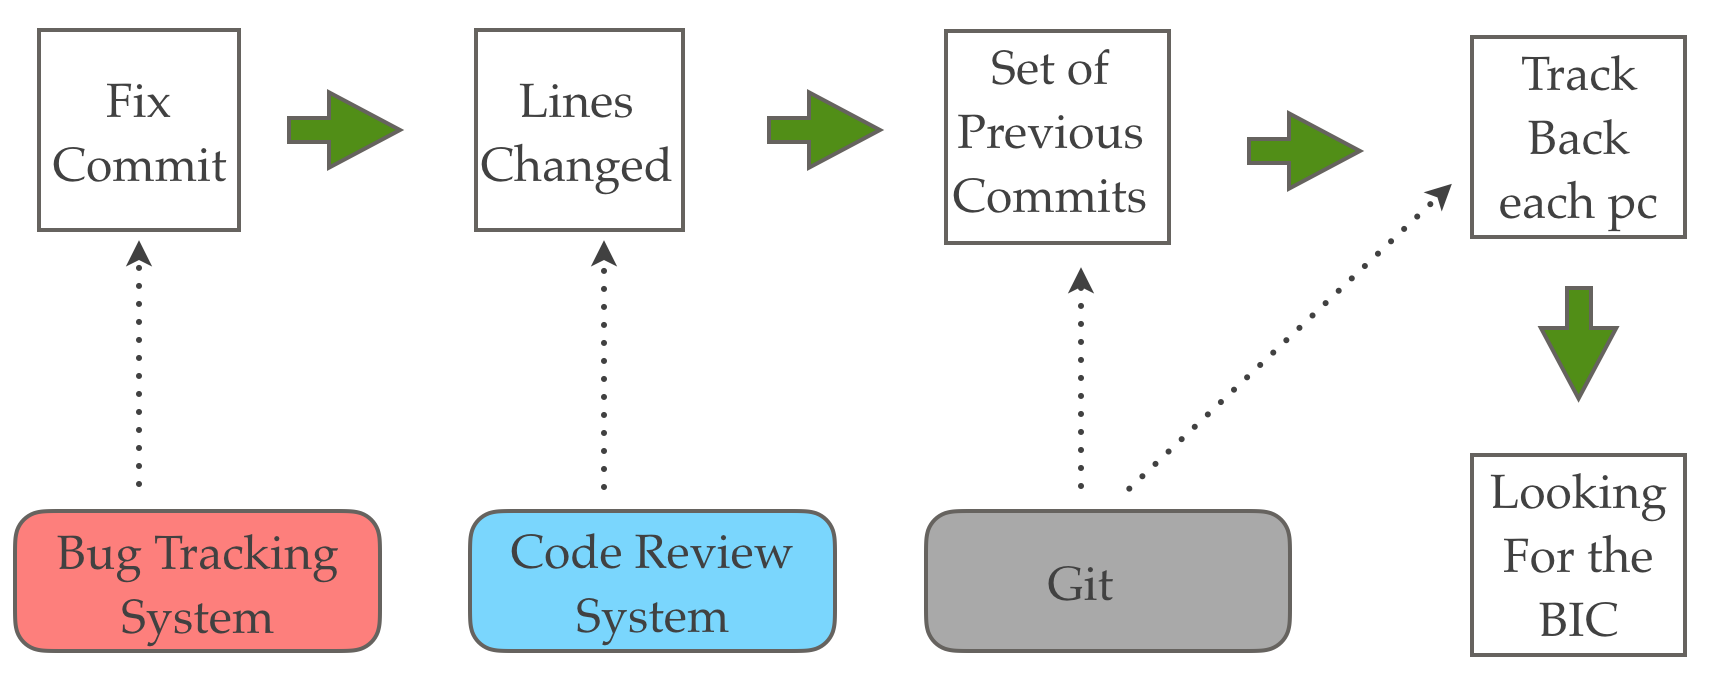
\includegraphics[width=\columnwidth]{methodology.png}
\caption{The methodology diagram, starting with the analysis of a fix commit and finishing with the value of the metrics}
\label{fig:methodology}       % Give a unique label
\end{figure}

The following list is a detailed description of the steps: 

\begin{enumerate}
		\item Find the fixing commit of each bug report.
		\item Find the lines that this commit added, modified or deleted to solve the bug.
		\item Obtain, for each of those lines, the commit that added, modified or deleted these lines previously. The result is the previous commit for each line.
		\item Analyze which one of the previous commits was the BIC. In the case where none of them was the cause of the bug, track back each previous commit until the line causing the failure can be found in some of the previous commits. In the case of only new lines were added to the fixing commit, we analyzed the nearby commits to those lines looking whether in any of them the developer \emph{forgot} to add these lines. Notice that SZZ algorithm discards the fixing commits with only new lines.
		\item Extract the date when the fixing commit, the BIC and the bug report was submitted, as well as the author of each of the commits to calculate our metrics.	
\end{enumerate} 


\subsection{Metrics}

To compute all the metrics used in this study, we need to identify the BIC. Once we have it, we are able to measure exactly all the time values we want.  

Next, we describe the metrics. Notice that the value of all these metrics has been calculated in days: 

\begin{itemize}
		\item \emph{Experience Until Bug Introducing Change} (EuBIC): The time of experience that presents the author of the BIC at the moment of doing the commit. The experience is measured from the first time that the author committed some code to the project until (s)he introduced the commit with the buggy line.
		\item \emph{Time To Notify} (TTN): This value measures the time since the commit inserted the bug was merged into he master branch until some developer notified the unexpected behavior and reported it. 
		\item \emph{Time To Fix} (TTF): It refers to period from the notification of a bug report to when it was closed with a fixing commit.
		\item \emph{Bug Fixing Time} (BFT): It measures the time from the date of the BIC and the fixing commit date. This time is calculated as the addition of the TTN and TTF time.
\end{itemize} 

Figure~\ref{fig:metrics} provides a visual explanation of the various metrics proposed in this paper. \grex{Explain the figure with an example}. As example, after analyzing the bug report \#13334 we obtain that the fix commit id is $c6da8d5e1$ and the BIC is $c73fff7$. Thus, extracting all the meta-data of theses commits we obtain the date and the author of each commit where the bug report was done on 4\textsuperscript{th} September 2015, the fixing commit was done on 15\textsuperscript{th} September 2015 and the BIC was inserted on 13\textsuperscript{th} July 2015 by a developer with almost 3 years of experience in the project. Hence, at this example the values of the metrics under study are:  TTN is 54 days, the TTF is 11 days the EuBIC is 1097 days and the BFT is 65 days.
\begin{figure}[ht]
\centering
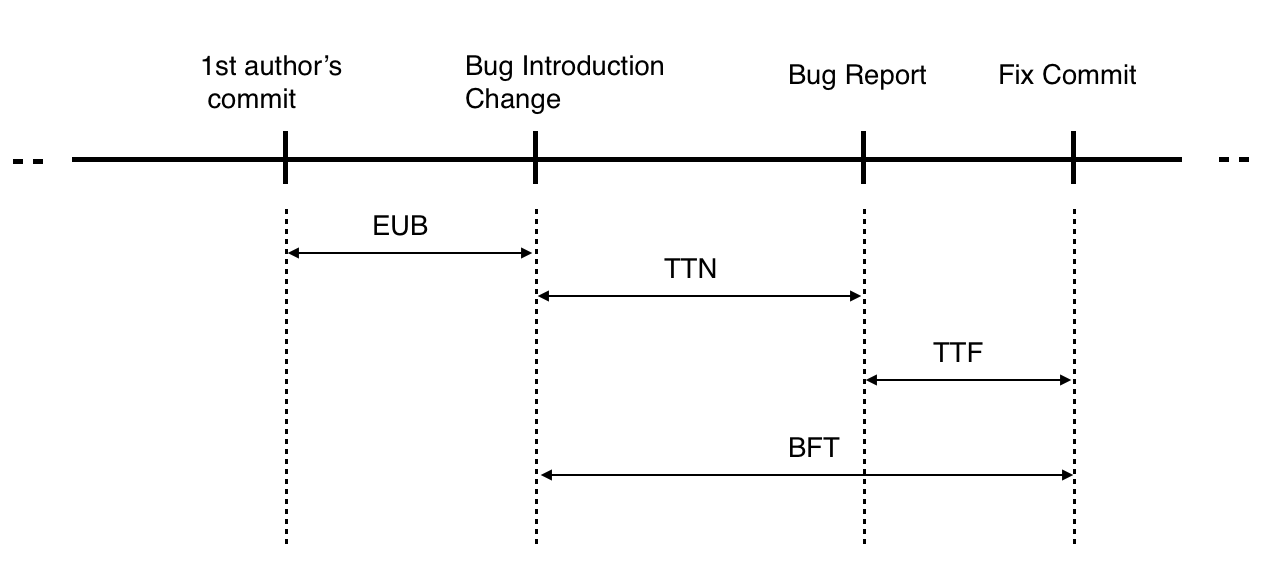
\includegraphics[width=\columnwidth]{metrics.png}
\caption{ Span period of the metrics: Experience Until Bug Introducing Change (EuBIC),  Time To Notify (TTN), Time To Fix (TTF), Bug Fixing Time (BFT) }
\label{fig:metrics}       % Give a unique label
\end{figure}

Until now, all the values have been calculated using the exact location of the BIC, but the SZZ algorithm does not locate the precise commit in which the bug was introduced, and its outcome could be a a set of commits among which the \emph{real} BIC may or not be. To compare our results with the ones obtained after using the SZZ algorithm, we select the earliest commit which introduced the bug to the bug-fixing commit as in prior works~\cite{eyolfson2011time}. In addition, we must discard those fixing commits with only new lines since SZZ algorithm removes them from the analysis.

\section{Evaluation}
\label{sec:evaluation}

We have validated our methodology analyzing tickets from two different projects written in different programming languages. Nova uses a dynamic language, whereas ElasticSearch uses a static language. Thus, we may study the dependency of the TTN with the programming language that the project is using.

Nova belongs to OpenStack project which is a cloud computing platform with a huge developing community (more than 5,000 developers) and significant industrial support from several major companies such as Red Hat, Intel, IBM, HP, etc. The source code of Nova is written in Python and was particularly of interest because it is continuously evolving due to its very active community. Currently it has more than 44,000 commits with more than 2 million lines of code and around 1,000 contributors\footnote{\url{http://activity.openstack.org/dash/browser/repository.html?repository=nova.git&ds=scm}}. All its code is hosted and available at GitHub\footnote{\url{https://github.com/openstack/nova}} and it works with git\footnote{\url{https://git-scm.com/}} as the source code management, Launchpad\footnote{\url{https://launchpad.net/}} as the issue tracking system and Gerrit\footnote{\url{https://www.gerritcodereview.com/}} as the code review system.

ElasticSearch is a distributed FLOSS search and analytics engine written in Java. It has a lower number of commits and contributors than OpenStack, 26,000 commit and 764 contributors. Its policy of labelling an issue as bug report is very strict, thus we could be sure that the tickets analyzed are \emph{real} bug reports. All its code is hosted at GitHub\footnote{\url{https://github.com/elastic/elasticsearch/}} and it has been used such as issue tracking system and pull request system in this project.

In this study we used a data set created in a prior research work where we analyzed manually and in detail a total of 76 bug fixing commits of real bug reports, looking in each one for the bug introducing change that caused the failure, presented at the Doctoral Consortium at the 12\textsuperscript{th} International Conference on Open Source Systems~\cite{crowston2016proceedings}\grex{citation needed}\gema{done!}. Thus, once we have the commit that induced the later fix, we calculate the values of the TTN, EuBIC, TTF and the authors of the fixing commit, the bug report, and the bug introducing change.  

\grex{We should have a replication package with data and scripts}
\gema{http://gemarodri.github.io/Reprodu-Package/ I have to write more info here, but here we have all the data and the detailed information }

\section{Results}
\label{sec:results}

We have analyzed exactly the values of the TTN, the EuBIC, and the TTF in the 76 bug fixing commits, 39 belong to Nova and 37 belong to ElasticSearch. In addition, we compare these values with the values resulting of SZZ.

Table~\ref{tableNova} and Table~\ref{tableES} \gema{all the references to tables say Table V instead of their correct number, I don't know what is wrong} show the mean of the Time To Notify (TTN), the Time To Fix (TTF) and the Bug Fixing Time (BFT) variables computed in Nova and ElasticSearch project, respectively,  using our methodology \emph{Manually} and the SZZ algorithm. 

\begin{table}[!t]
% increase table row spacing, adjust to taste
\renewcommand{\arraystretch}{1.3}
\label{tableNova}
\centering
\caption{Mean in days of the TTN, TTF, BFT in Nova project}
% Some packages, such as MDW tools, offer better commands for making tables
%% than the plain LaTeX2e tabular which is used here.
\begin{tabular}{|c||c||c||c| }
\hline
  & TTN & TTF & BFT \\
\hline
Manually & 432 & 65 & 497 \\
\hline
SZZ & 260 & 52 & 312\\
\hline
\end{tabular}
\end{table}

\begin{table}[!t]
% increase table row spacing, adjust to taste
\renewcommand{\arraystretch}{1.3}
\label{tableES}
\centering
\caption{Mean in days of the TTN, TTF, BFT in ElasticSearch project}
% Some packages, such as MDW tools, offer better commands for making tables
%% than the plain LaTeX2e tabular which is used here.
\begin{tabular}{|c||c||c||c| }
\hline
  & TTN & TTF & BFT \\
\hline
Manually & 312 & 14 & 326 \\
\hline
SZZ & 135 & 16 & 151\\
\hline
\end{tabular}
\end{table}

Figure~\ref{fig:meansOfNova} and Figure~\ref{fig:meansOfES} shows the TTN as well as the TTF and the EuBIC in both projects using box plots. For example, to notify 50\% of the bugs requires approximately 158 days in ElasticSearch and 336 days in Nova. Whereas the median is around 350 days in Nova and almost 200 days in ElasticSearch.  

\begin{figure}[ht]
\centering
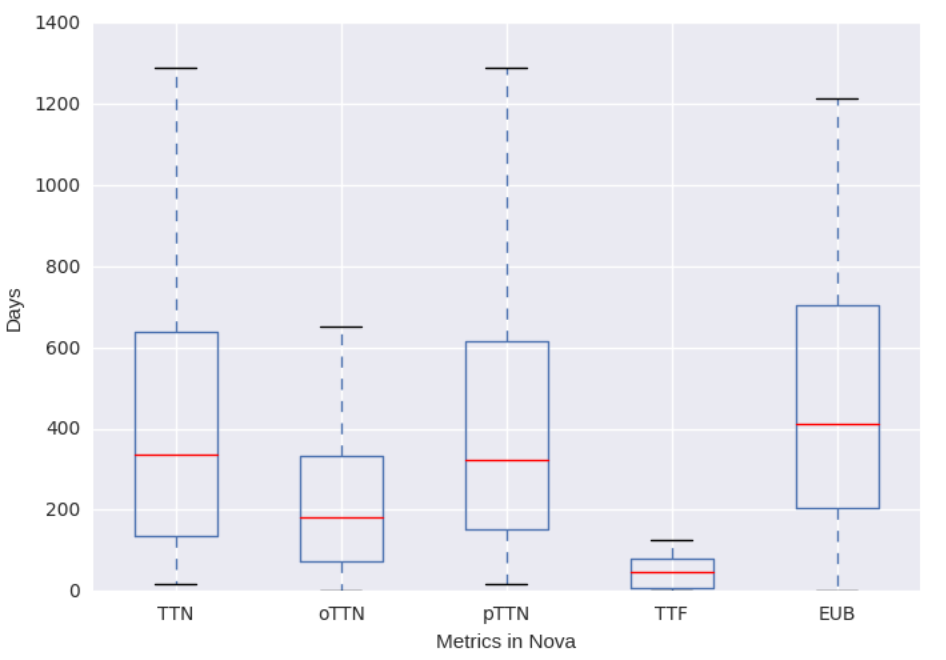
\includegraphics[width=\columnwidth]{boxplotNova.png}
\caption{The boxes indicate 50\% of TTN, oTTN, pTTN, TTF and EuBIC (25\% to 75\% quartile) in Nova project. The middle line in boxes indicates the median value}
\label{fig:meansOfNova}       % Give a unique label
%\caption{Box-Plot in Nova}
%\label{fig:graph4}       % Give a unique label
\end{figure}

\begin{figure}[ht]
\centering
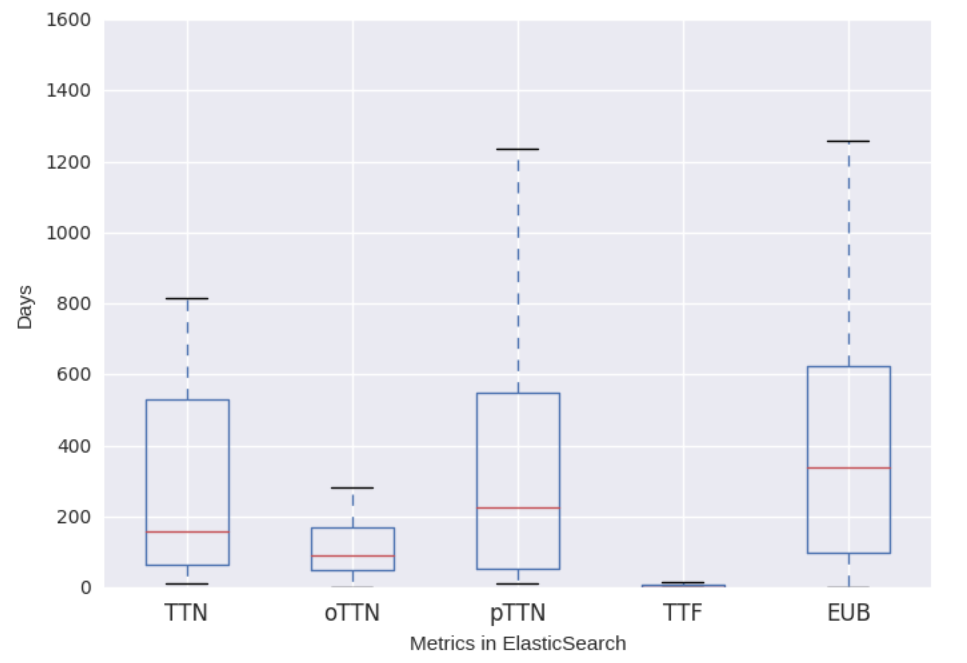
\includegraphics[width=\columnwidth]{boxplotES.png}
\caption{The boxes indicate 50\% of TTN, oTTN, pTTN, TTF and EuBIC (25\% to 75\% quartile) in ElasticSearch project. The middle line in boxes indicates the median value}
\label{fig:meansOfES}       % Give a unique label
%\caption{Box-Plot in ES}
%\label{fig:graph5}       % Give a unique label
\end{figure}

The Figure~\ref{fig:correlation} shows the correlation between the metrics under analysis in Nova project. It shows a moderate negative correlation, $-0.56$, between the experience of the author introducing the bug and the Time To Notify. The value of this correlation in ElasticSearch project is $-0.383$, that means a weaker correlation than the one shows in Nova project and we decided not display the graph.

\begin{figure}[ht]
\centering
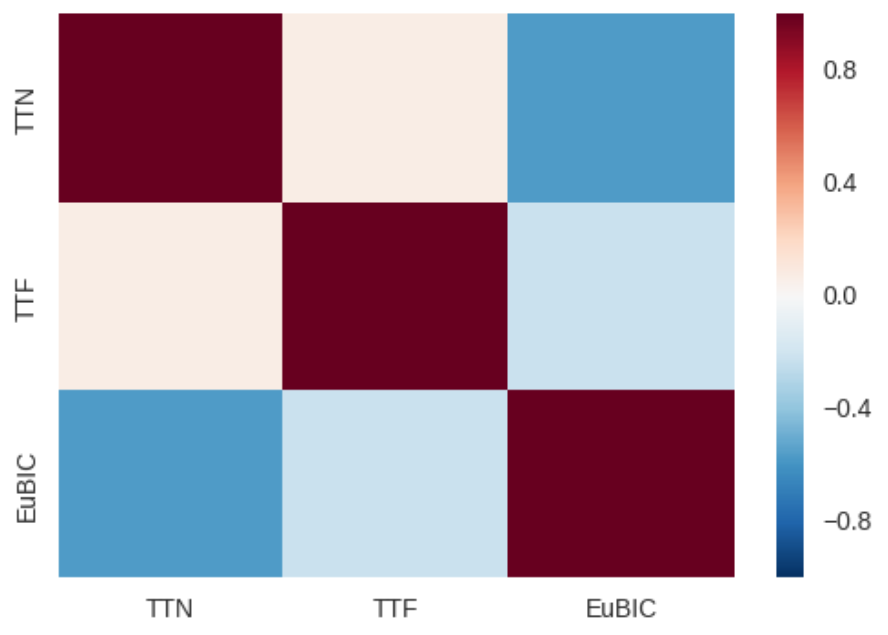
\includegraphics[width=\columnwidth]{correlationMatrix.png}
\caption{Correlation Matrix of the variables measured in Nova project. Correlation coefficients are coloured according to the value where the white means a correlation value of 0, the red tone increases with the grade of positive correlation and the blue tone decreases with the grade of negative correlation }
\label{fig:correlation}       % Give a unique label
\end{figure}

The Figure~\ref{fig:graph} shows the correlation distribution that each variable has with the others in Nova project. While we can suspect a negative inclination in the relationship between TTN and EuBIC which indicates how closely this two variables are related, the plot for TTN or EuBIC against TTF does not indicate such tendency.

\begin{figure}[ht]
\centering
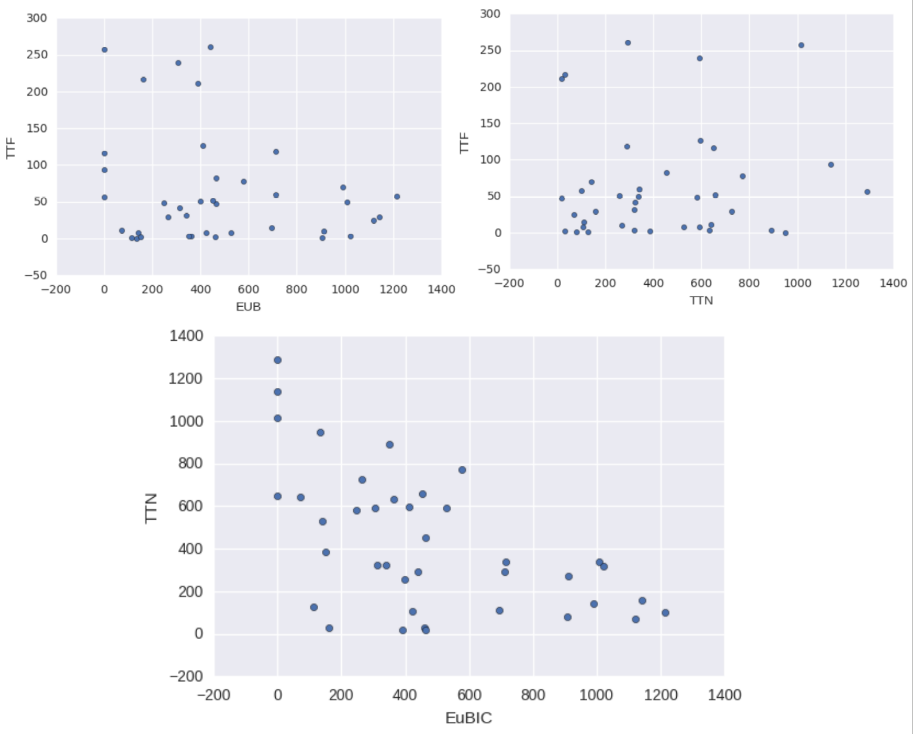
\includegraphics[width=\columnwidth]{DistributionNova_b.png}
\caption{ Relationship of the metrics each other in Nova project. \grex{We should make these figures bigger}
\gema{Better?}}
\label{fig:graph}       % Give a unique label
\end{figure}

On the other hand, the Figure~\ref{fig:graph1} also shows how the variables are related each others in the ElasticSearch project. In this project, it is more difficult to notice the negative inclination in the graph comparing TTN and EuBIC but, although the matrix correlations showed a very weak value for this comparison in this project, we may see the small tendency in the graph. On the contrary, the plot for TTN or EuBIC against TTF does not indicate such tendency.
\begin{figure}[ht]
\centering
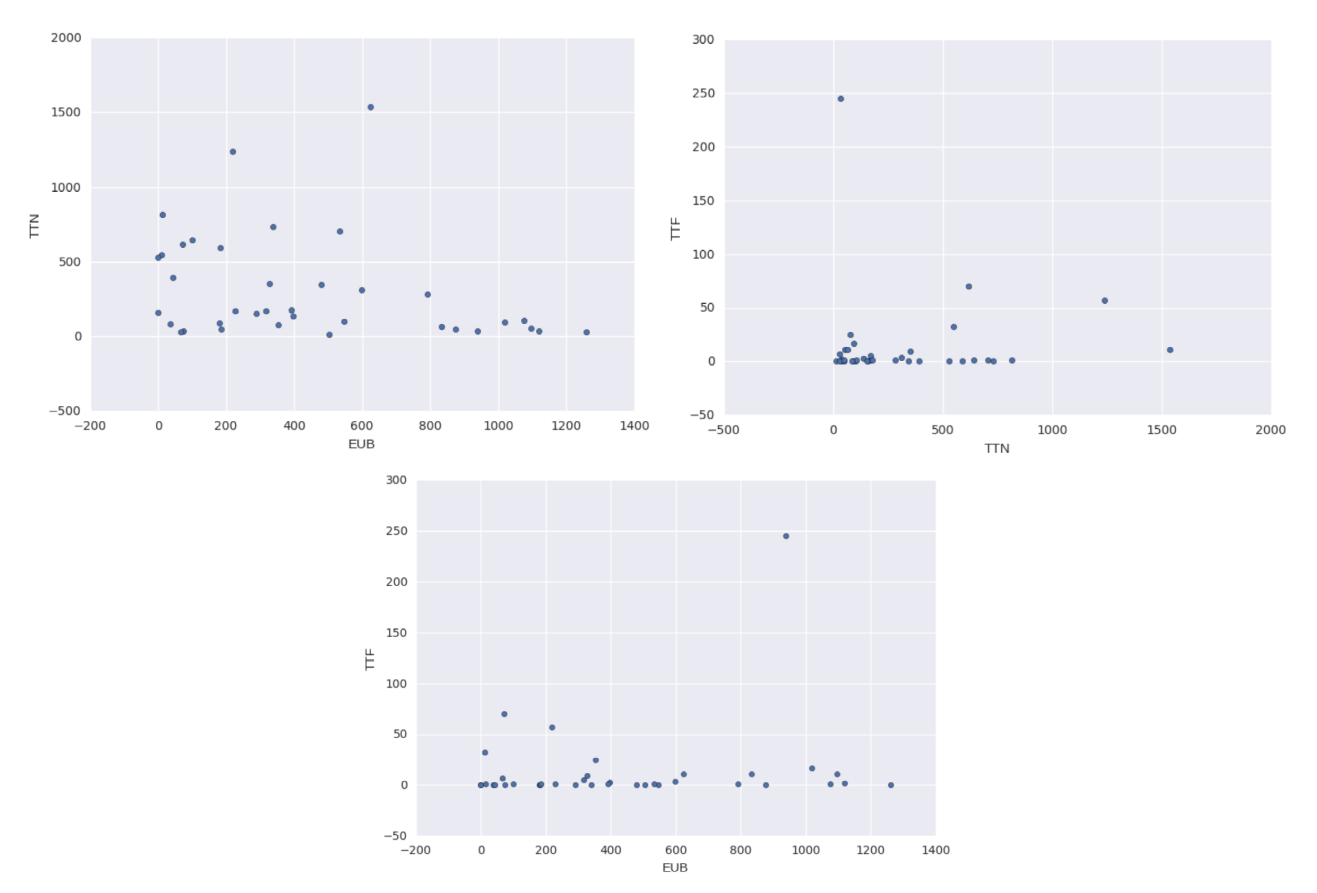
\includegraphics[width=\columnwidth]{DistributionES_b.png}
\caption{Relationship of the metrics each other in ES project. \grex{We should make these figures bigger}}
\label{fig:graph1}       % Give a unique label
\end{figure}


To give context about the possible reasons for the value of the TTN in both project, we observed whether the persons introducing the BIC, reporting the bug or fixing it were the same person or not. The Table~\ref{tableII} and Table~\ref{tableIII} show the percentage of people in ElasticSearch and Nova respectively who: (1) notified and fixed the bug, (2) Introduced the BIC, notified the bug and fixed it, (3) Introduced the BIC and notified the bug, or (4) Introduced the BIC and fixed the bug.
\begin{table}[!t]
% increase table row spacing, adjust to taste
\renewcommand{\arraystretch}{1.3}
\label{tableII}
\centering
\caption{Percentage of same people introducing, notifying and fixing the bugs in ElasticSearch project}
% Some packages, such as MDW tools, offer better commands for making tables
%% than the plain LaTeX2e tabular which is used here.
\begin{tabular}{|c||c||c||c||c| }
\hline
  & Notify-Fix & Introduce-Notify-Fix & Introduce-Notify & Introduce-Fix \\
\hline
Yes & 16 (43\%) & 10 (27\%) & 11 (30\%) & 16 (43\%) \\
\hline
No & 21 (57\%) & 27 (73\%) & 26 (70\%) & 21 (57\%) \\
\hline
\end{tabular}
\end{table}

\begin{table}[!t]
% increase table row spacing, adjust to taste
\renewcommand{\arraystretch}{1.3}
\label{tableIII}
\centering
\caption{Percentage of same people introducing, notifying and fixing the bugs in Nova project}
% Some packages, such as MDW tools, offer better commands for making tables
%% than the plain LaTeX2e tabular which is used here.
\begin{tabular}{|c||c||c||c||c| }
\hline
  & Notify-Fix & Introduce-Notify-Fix & Introduce-Notify & Introduce-Fix \\
\hline
Yes & 30 (77\%) & 5 (13\%) & 5 (13\%) & 7 (18\%) \\
\hline
No & 9 (23\%) & 34 (87\%) & 34 (87\%) & 32 (82\%) \\
\hline
\end{tabular}
\end{table}
\section{Discussion}
\label{sec:discussion}

After analyzing several fixing commit in this study, we have realized that the \emph{real} Time To Notify a bug differs to the one computed using an algorithm such as SZZ, the percentage of times that this metric concurs is 36\% in Nova and 24\% in ElasticSearch. The TTN computed using SZZ is almost the half that the one calculated using our methodology. The principal reasons of this results are (1) The bug fixing commit with only new lines are discarded by SZZ and, (2) The assumption done by SZZ where the earliest commit to the bug fixing commit is suspicious to be the BIC.


The median time to notify a bug is almost 200 days in ElasticSearch and about 350 days in Nova. To calculate the median time of bug fixing in each project we add to the TTN values the median time to fix a bug per project, it arise that bug fixing time in ElasticSearch does not have any variation whereas it is increased in Nova reaching to almost 400 days. In addition, using the range of BFT which varies from 100 to 200 calculated by Kim and Whitehead in ~\cite{kim2006long}, we notice that none of the projects are on the range. The explanation of that is because to calculate the bug fixing time they use SZZ to locate the suspicious commit to be the BIC.

\vspace{0.2cm}
\fbox{\begin{minipage}{24em}
\textbf{$H_0$: The real value of the Time to Notify (TTN) a bug in both projects differs from the value calculated using SZZ } 
\end{minipage}}
\vspace{0.1cm}

One of our findings is the negative correlation that Nova presents between two of the variables compared. This correlations implies that the TTN increases when the EuBIC is lower, meaning that one of the reasons why the TTN is high some times could be that the author who injected the bug in the code had few experience in the project at this moment.

\vspace{0.2cm}
\fbox{\begin{minipage}{24em}
\textbf{ $H_2$: The experience of the author who inserted the bug in the source code and the Time To Notify it are correlated} 
\end{minipage}}
\vspace{0.1cm}

On the contrary, the results denote that the hypothesis $H_1$ and $H_3$ are positives. 

\vspace{0.2cm}
\fbox{\begin{minipage}{24em}
\textbf{ $H_1$, $H_3$: The results do not show any correlation between the Time To Fix with the Time to Notify or the experience of the author who inserted the bug in the source code} 
\end{minipage}}
\vspace{0.1cm}

A interesting question to answer was \emph{Do the authors of the BIC fix/notify theirs bugs?}. In ElasticSearch a 43\% of the developers
 that opened a bug report notifying the wrong behavior of the system, then fixed the bug. In addition, the author of the BIC was the person who afterwards fixed it in a 43\%. Whereas in Nova, the percentage of developers reporting and fixing the bug is higher, a 77\%. But, it was not common that the authors of the BIC fixed their own bugs, only 18\% of the developer did it. One possible reason to explain the lower percentage of authors who fixed their bugs may be because they were no longer in the project after the bug was reported. But in fact, the number of authors who abandoned the project before the bug was reported were only one in ElasticSearch and two in Nova, so in the data analyzed there must be other reasons more important that proprietary of the code to fix a bug. On the contrary, the higher percentage of developers notifying and fixing the bugs may be due to when they are reporting the bug, they already know how to fix it, and this might have and impact reducing the time to fix a bug. 

Finally, the analysis of the Time To Notify a bug has demonstrated that is a valuable metric which has a correlation with the experience of the author who inserted the BIC in the source code and which is not being measured correctly. As solution, the bug tracking system has to evolve providing a field to write which is the bug introduction commit according to the developer who fixed the bug. There is no one more qualified at this moment that knows where and when the bug was caused, that way the researchers might trust in that commit and build a better models that measure the effort of a software.  

\section{Threats to validity}
\label{sec:threats}
The limited sample size of tickets used in this research is the major threat to its validity. It is relatively high considering that the analysis was done manually and in detail to reach reliable results, but there is a long way to get a representative sample from a variety of free/open source systems, or software projects at large. Our analysis requires a lot of human effort, so increasing meaningfully the number of tickets is difficult. However, it should be noted that our numbers are the order of magnitude of similar studies: for instance Hindle's \emph{et al.} ~\cite{hindle2008large} article on large commits, considered 100 commits.

Other internal threats to validity are:

\begin{itemize}
    \item We are only using part of the information that the tickets provide, like comments and text. There could be some patterns that can be found in other parts of the information, but we think that this information is enough to determine where the bug introducing change is, due to the comments of the developers in the ticket give several information about what is failing in the code.
    \item In some cases, when only new code was added by the bug fixing commit, researchers may have some problems to compare their TTN with the SZZ because of SZZ does not considered the new additions in the fixing commits. 
    \item The experience of the developer calculated from its first commit in the system may not be the best definition to indicate the experience of the author due to a old contributor could have less commit and as a consequence less experience in the project that a new active contributor who is committing all time.
\end{itemize}

The most important external threats, most of them related to peculiarities of the Nova project, are:

\begin{itemize}
    \item OpenStack is a special project with a very rapid evolution, and a very active community of developer and ElasticSearch is relatively new project with a strong criteria in the bug fix activity. Maybe, in other projects with less commits per year, results may be totally different.
    \item The programming languages analyzed at this research are Python and Java Script: It may happen that other programming languages present different results
\end{itemize}

\section{Conclusion and further research}
\label{sec:conclusions}

The studied we have performed in Nova and ElasticSearch has shown that the mean time to notify a bug in the system is higher than ten months when the location of the bug introducing change is known. Whereas using SZZ to calculate this metric this value is higher than five months.

Our study also shows a negative correlation between the TTN and the EuBIC, which may indicates that a higher time to notify a fewer experience of the author who created the bug. 

Once we have found this, it makes sense to explore, as future work, to which extent this happens in other projects with probably higher number of tickets and with a higher number metrics.

\section*{Acknowledgment}


We want to express our gratitude to Bitergia\footnote{\url{http://bitergia.com/}} for their open source tools to mining the repositories of the projects and the support they have provided when questions have arisen. Also, we acknowledge the Spanish Government, because some authors are funded in part by it, through project TIN2014-59400-R as well as the University the Victoria and University Rey Juan Carlos that have promoted the collaboration between Universities.

% trigger a \newpage just before the given reference
% number - used to balance the columns on the last page
% adjust value as needed - may need to be readjusted if
% the document is modified later
%\IEEEtriggeratref{8}
% The "triggered" command can be changed if desired:
%\IEEEtriggercmd{\enlargethispage{-5in}}

% references section

% can use a bibliography generated by BibTeX as a .bbl file
% BibTeX documentation can be easily obtained at:
% http://www.ctan.org/tex-archive/biblio/bibtex/contrib/doc/
% The IEEEtran BibTeX style support page is at:
% http://www.michaelshell.org/tex/ieeetran/bibtex/
%\bibliographystyle{IEEEtran}
% argument is your BibTeX string definitions and bibliography database(s)
%\bibliography{IEEEabrv,../bib/paper}
%
% <OR> manually copy in the resultant .bbl file
% set second argument of \begin to the number of references
% (used to reserve space for the reference number labels box)
%\begin{thebibliography}{1}

%\bibitem{IEEEhowto:kopka}
%H.~Kopka and P.~W. Daly, \emph{A Guide to \LaTeX}, 3rd~ed.\hskip 1em plus
%  0.5em minus 0.4em\relax Harlow, England: Addison-Wesley, 1999.

%\end{thebibliography}
\newpage

\bibliographystyle{abbrv}
\bibliography{sigproc} 


% that's all folks
\end{document}


